\subsection{Latency Development from 2022 to 2024} \label{sec:latency-wholerange}

It is in question whether and how Starlink latency has developed in the
timeframe of the data collection (January 2022 to June 2024). To determine
latency, we looked at TLS handshake latency. The data originates from the RIPE
Atlas TLS data that has been collected by built-in measurements (i.e.,
measurements that are continuously running in each individual probe in a fixed
time interval).

\begin{figure}
	\centering
	\begin{subfigure}[b]{0.49\linewidth}
		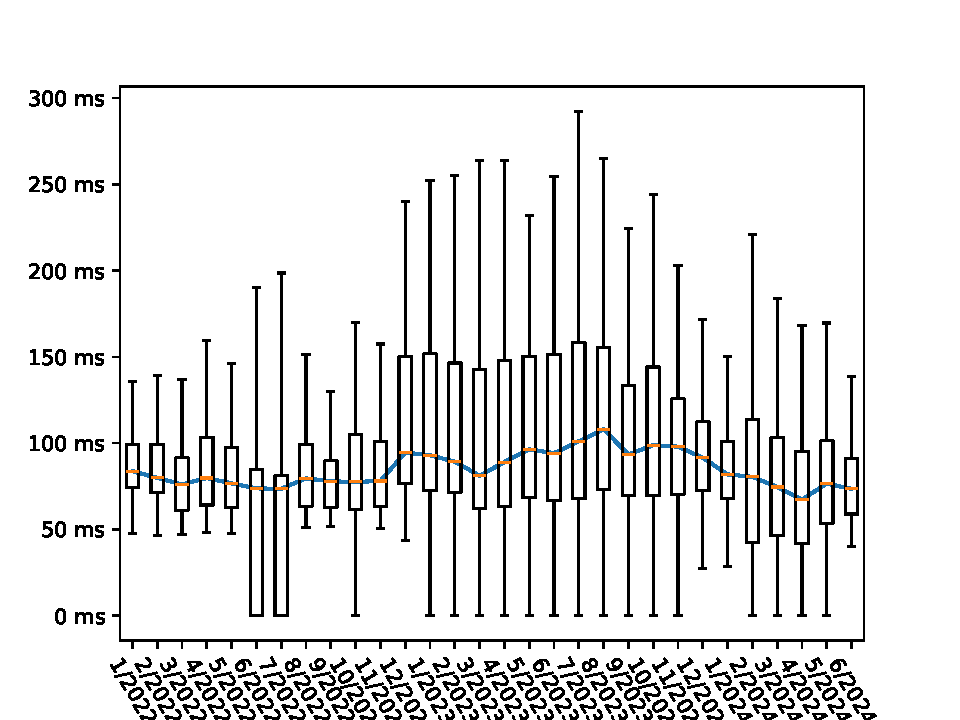
\includegraphics[width=\linewidth]{chapters/4-results/latency/img/latency_2022_to_2024_Germany.pdf}
		\caption{Germany}
	\end{subfigure}
	\begin{subfigure}[b]{0.49\linewidth}
		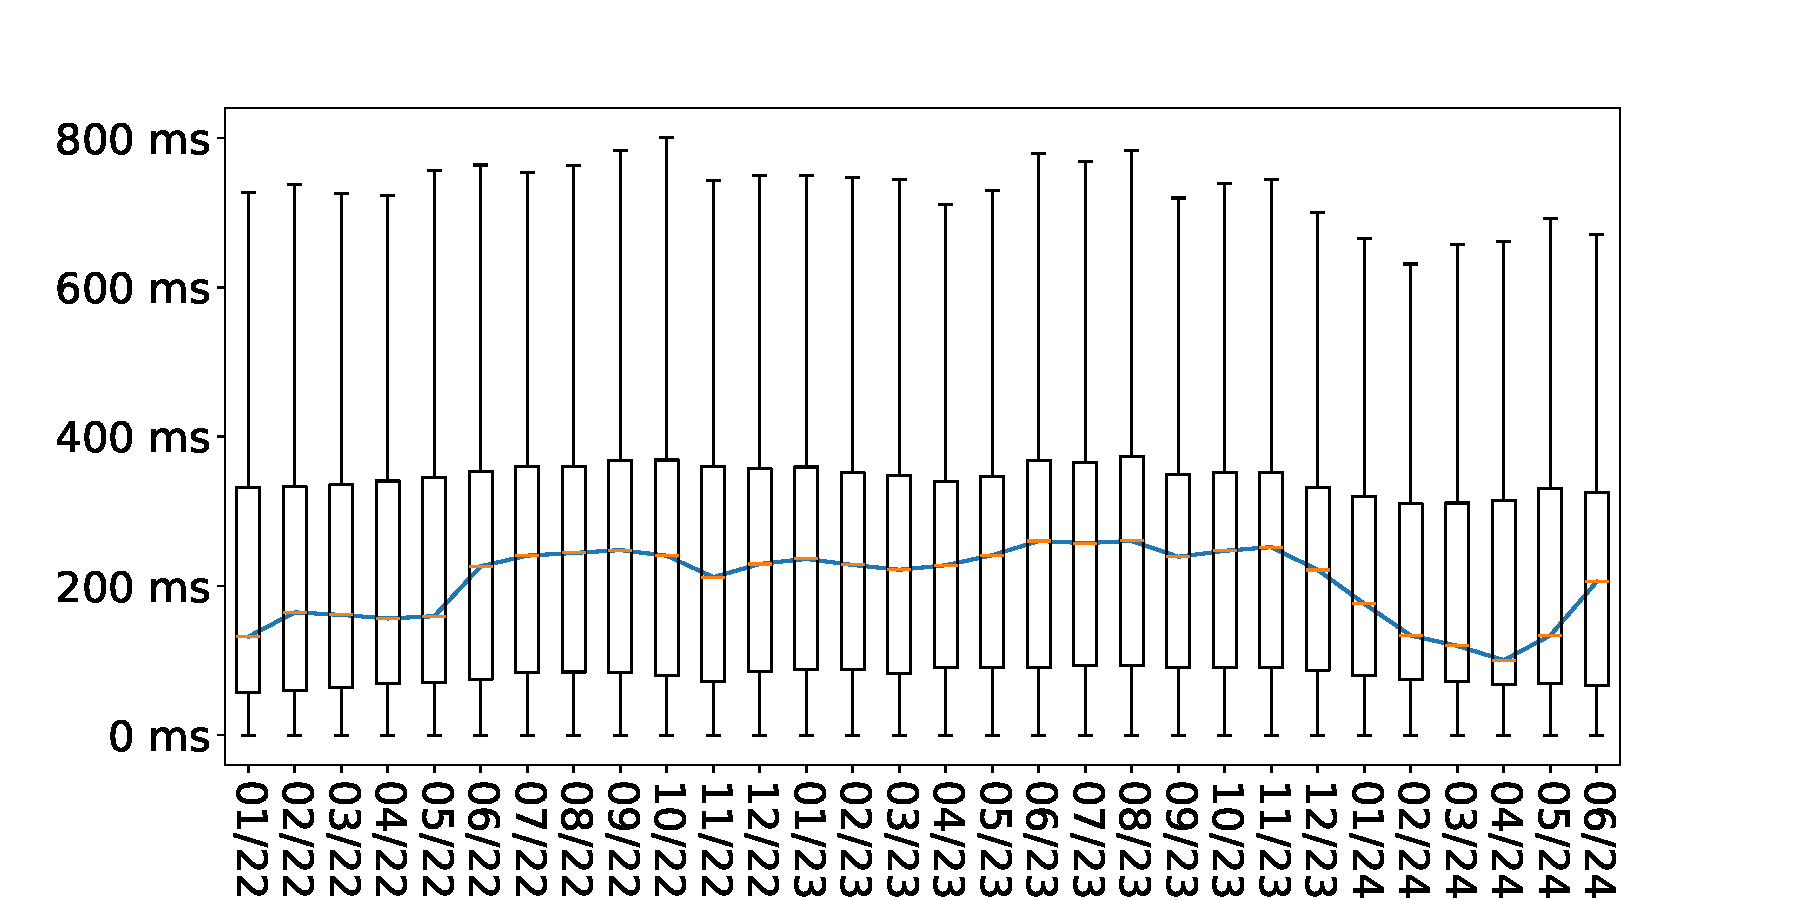
\includegraphics[width=\linewidth]{chapters/4-results/latency/img/latency_2022_to_2024_United States.pdf}
		\caption{USA}
	\end{subfigure}
	\begin{subfigure}[b]{0.49\linewidth}
		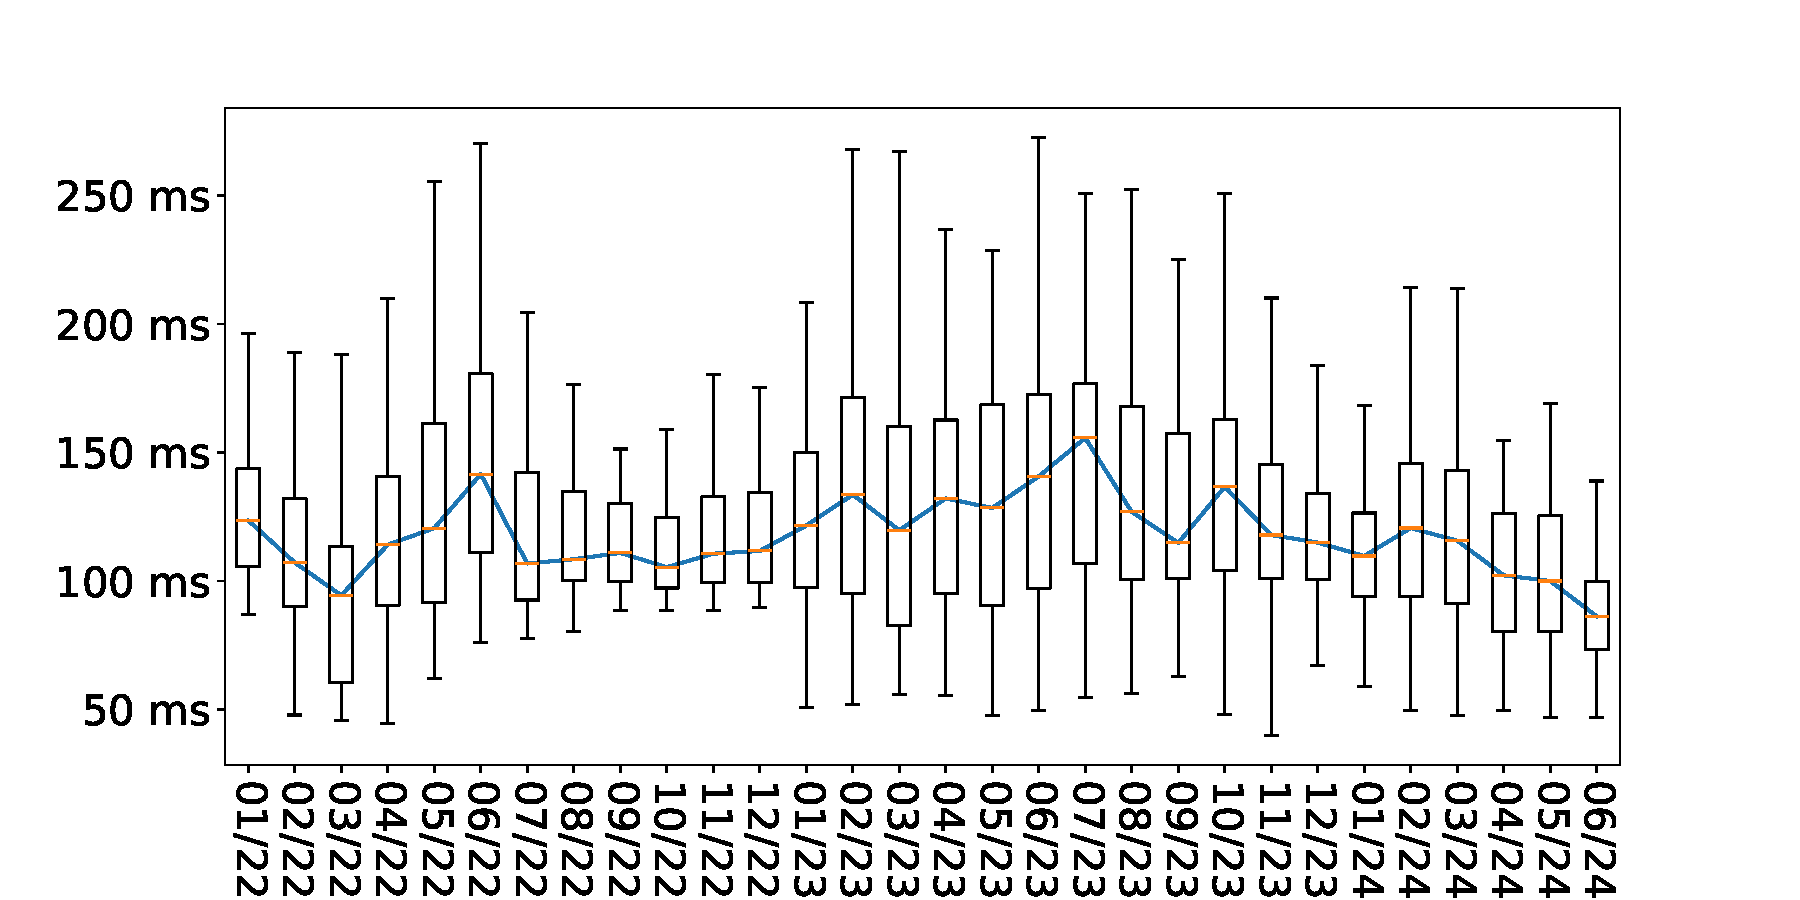
\includegraphics[width=\linewidth]{chapters/4-results/latency/img/latency_2022_to_2024_Poland.pdf}
		\caption{Poland}
	\end{subfigure}
	\begin{subfigure}[b]{0.49\linewidth}
		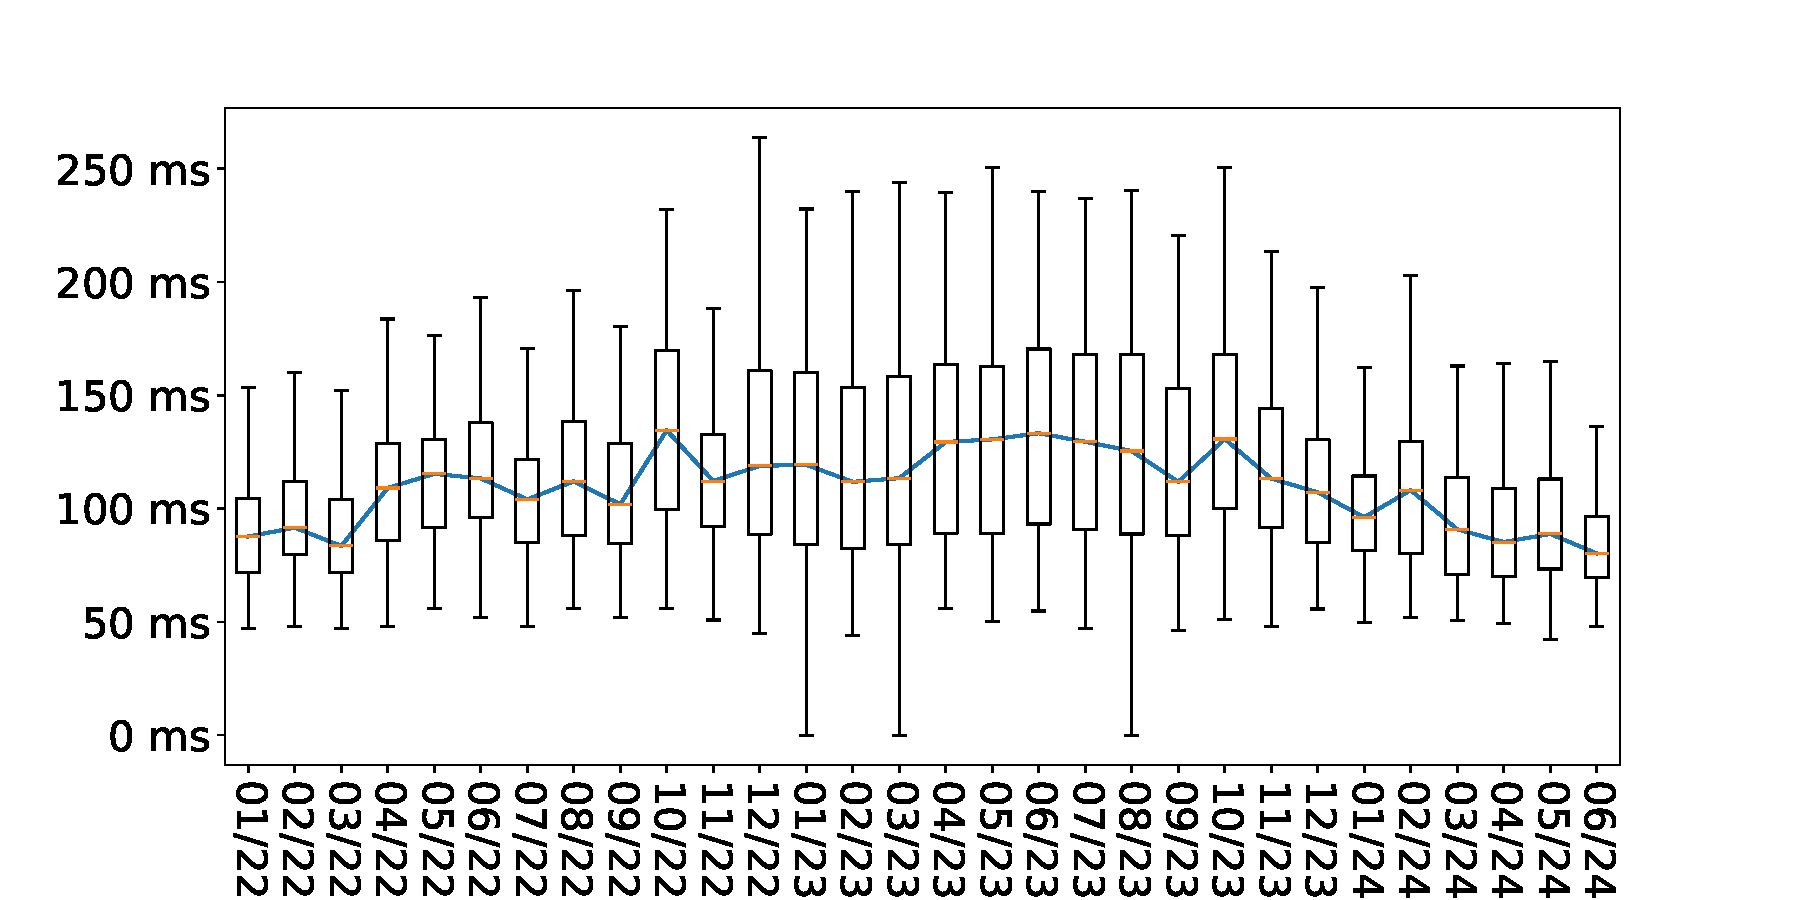
\includegraphics[width=\linewidth]{chapters/4-results/latency/img/latency_2022_to_2024_Austria.pdf}
		\caption{Austria}
	\end{subfigure}
	\caption{Latency History for Germany, the USA, Poland, and Austria in the period 01/2022 to 06/2024}
	\label{fig:latency_wholerange}
\end{figure}

\Cref{fig:latency_wholerange} shows the history of median TLS handshake
latencies from January~2022 until June~2024 for Germany, the United States,
Poland, and Austria\footnote{These countries were chosen due to the
	completeness of data}.

One can see that the median TLS handshake latency is usually at around 100 to
150~ms for most countries. However, the latency in 2022 was lower compared to
2023. Most of the countries observed show an upwards trend in the late months
of 2022 (most of the time in December). In the late months of 2023, the latency
starts to decline again. In the last couple of months until June 2024, we
observe an increase in latency once again. We assume the reason for the rise is
the congestion of the Starlink network. In the recent time, Starlink extended
their availability across more countries allowing more users, especially those
in countries with less networking infrastructure, to access the network. On the
contrary, Starlink also launched more satellites (2022: 3481, 2024: 6000+; see
\Cref{sec:satellite-constellations}) and added more \ac{GS}s which likely
reduces the congestion.

\begin{figure}[h]
	\centering
	\begin{subfigure}[t]{0.47\linewidth}
		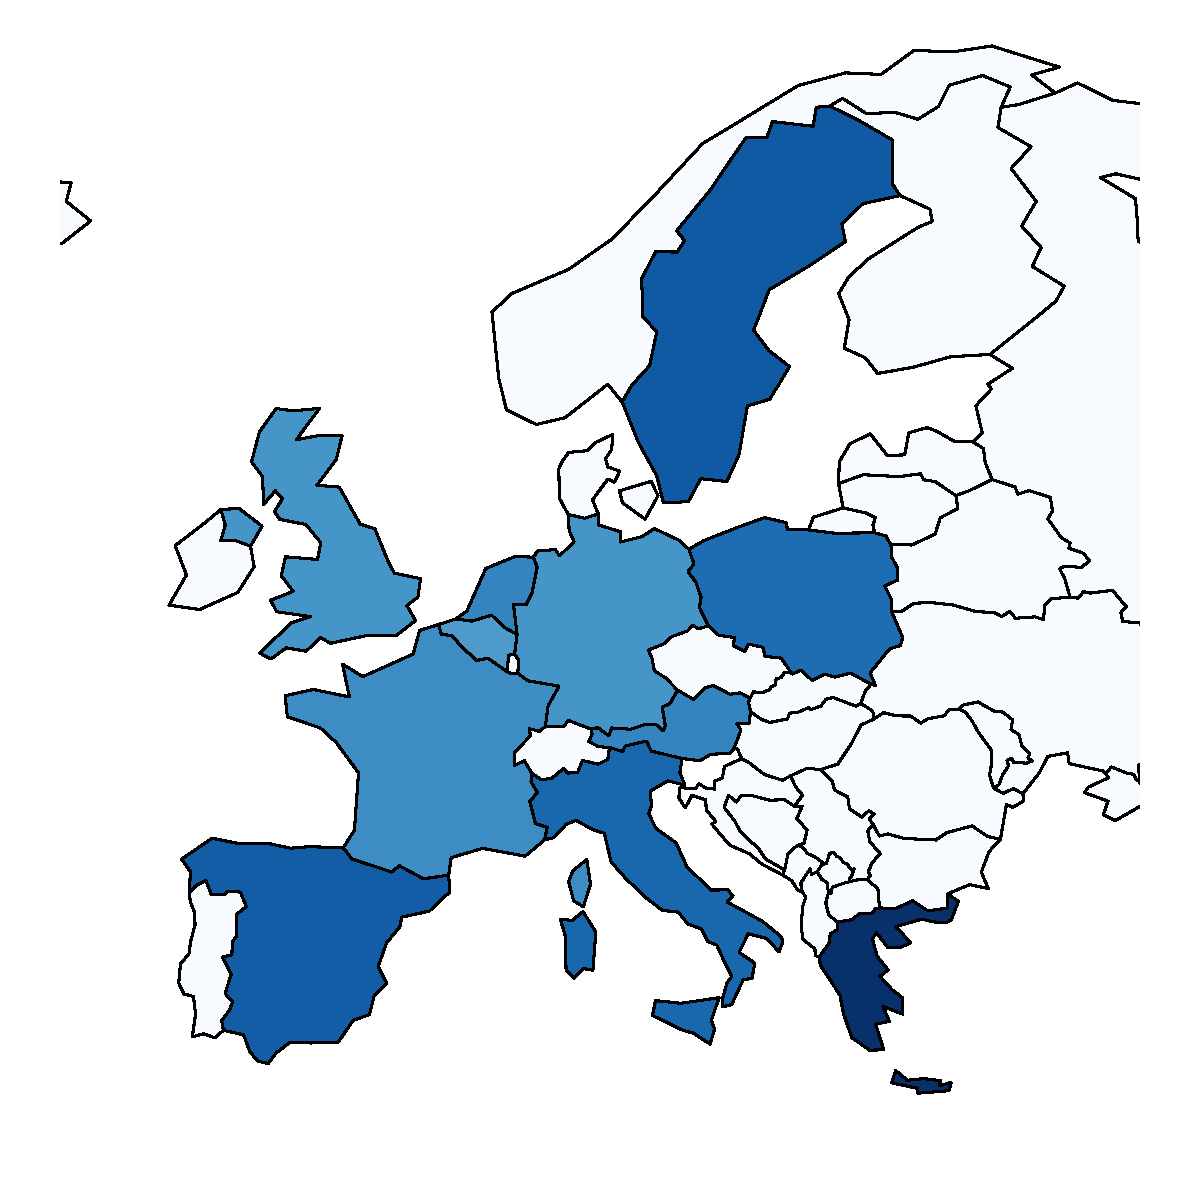
\includegraphics[width=\linewidth]{chapters/4-results/latency/img/heatmap-median-latencies-2024.pdf}
		\caption{Median}
	\end{subfigure}
	\begin{subfigure}[t]{0.47\linewidth}
		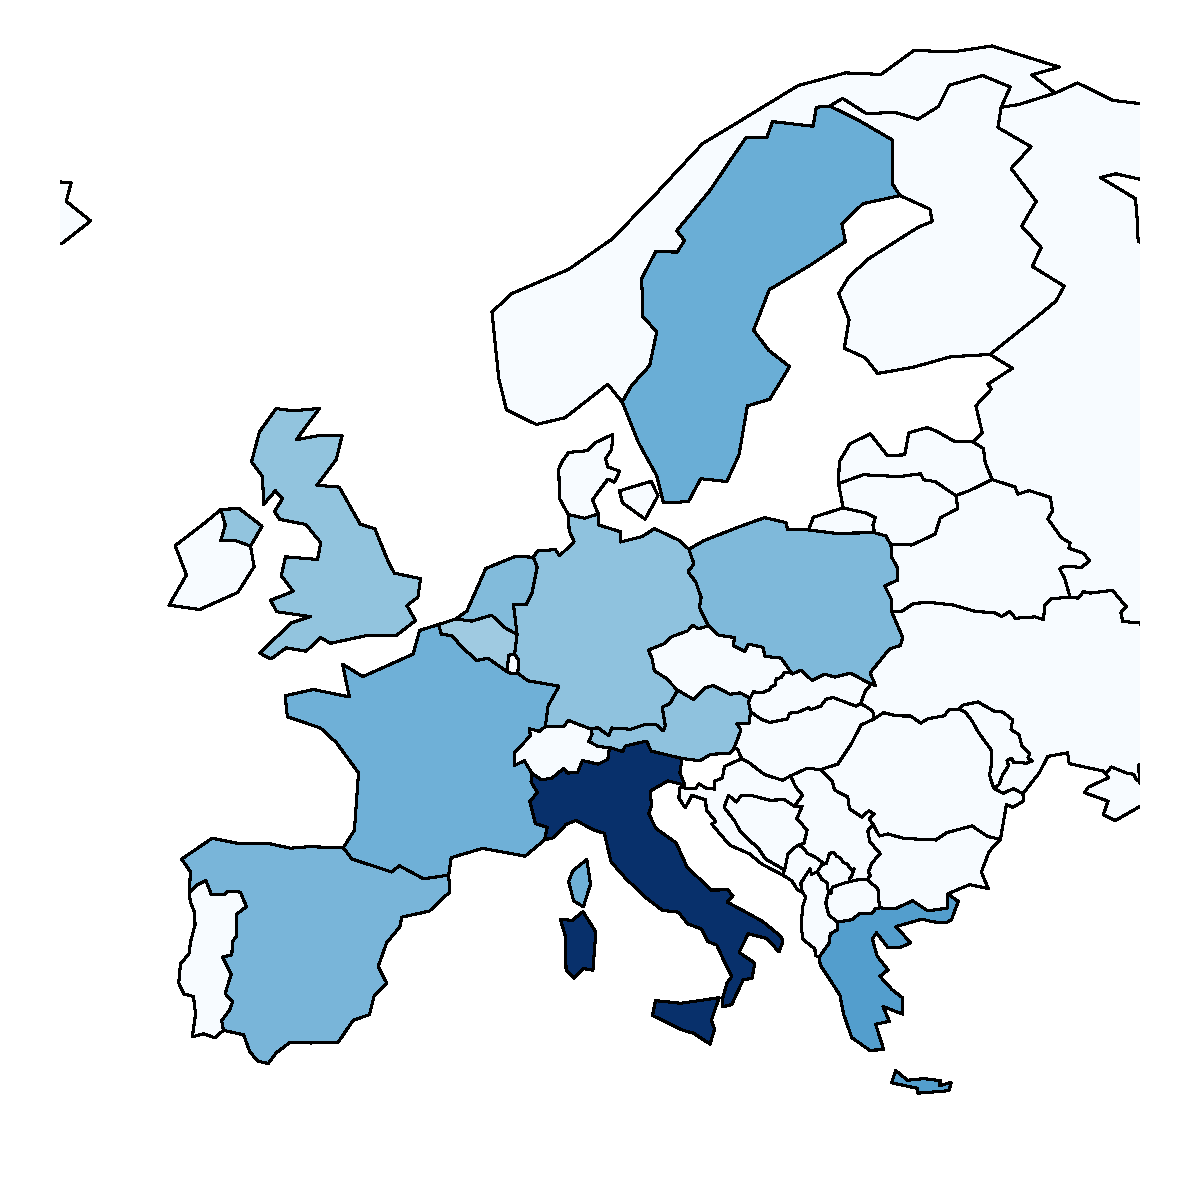
\includegraphics[width=\linewidth]{chapters/4-results/latency/img/heatmap-average-latencies-2024.pdf}
		\caption{Average}
	\end{subfigure}
	\caption{Heatmap of Median and Average Latencies in 2024 in Europe.}
	\label{fig:heatmap-latencies-europe}
\end{figure}

\Cref{fig:heatmap-latencies-europe} shows the median and average TLS handshake
latencies in European countries. It shows that the north-west of Europe
experiences the best latencies, likely due to the presence of various \ac{GS}s.
The southern and eastern European countries experience worse latencies.
Especially Greece has a high median latency. A cause could be the absence of
\ac{GS}s in the east-european region. Italy on the other hand side experiences
a high average latency, even with \ac{GS}s being present in the country.

Looking at the CDFs of the USA and Canada results in a similar observation.
\Cref{fig:latency-cdfs-1} illustrates the CDF plots for 2022 -- 2024 for the
USA and Canada. We observe similar results for other countries, but only chose
the USA and Canada as it holds sufficient data for a conclusion.

In the CDFs, we observe a similar performance of 2022 and 2024, but a drop in
latency in 2023, similar to the conclusion we drew before. Also, the CDF is
continuous, up to a specific point, where it flattens, followed by a stronger
increase once again. This is similarly observed for curves of other countries
(e.g., for France and Germany in \Cref{fig:latency-cdfs-2}). This observation
suggests that there is a region of latencies that Starlink does not serve
equally. The specific location of the flattening behavior varies between
countries, but is usually located between 150 and 250 ms.

\begin{figure}
	\centering
	\begin{subfigure}[b]{0.8\linewidth}
		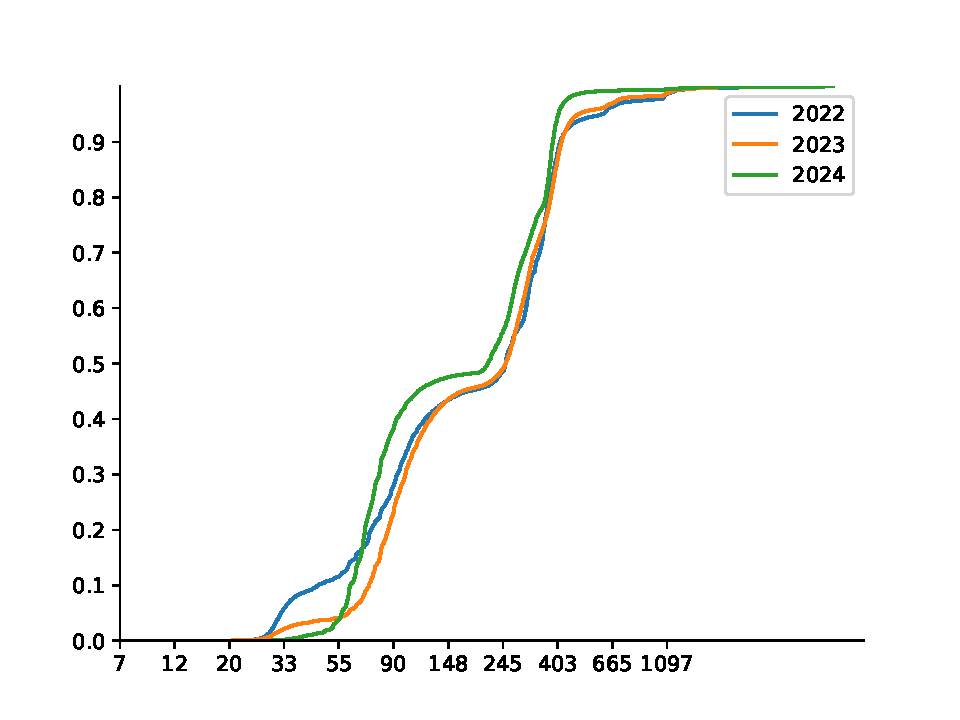
\includegraphics[width=\linewidth]{chapters/4-results/latency/img/cdf_latencies_of_starlink_probes_in_united_states.pdf}
		\caption{USA}
	\end{subfigure}
	\begin{subfigure}[b]{0.8\linewidth}
		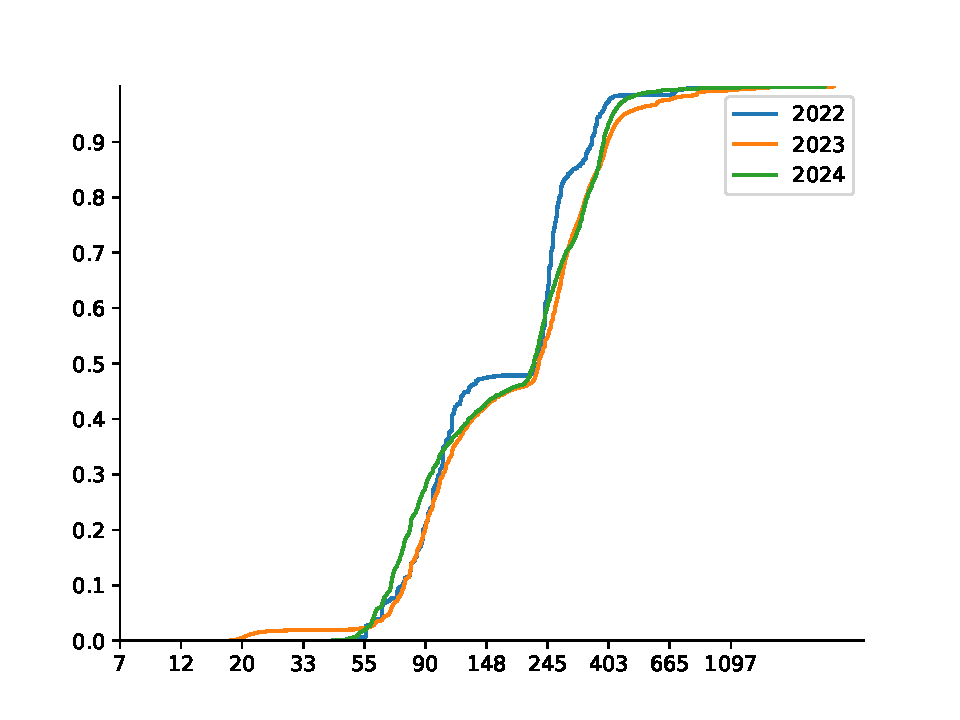
\includegraphics[width=\linewidth]{chapters/4-results/latency/img/cdf_latencies_of_starlink_probes_in_canada.pdf}
		\caption{Canada}
	\end{subfigure}
	\caption{CDF of Latencies in the USA and Canada}
	\label{fig:latency-cdfs-1}
\end{figure}

\begin{figure}
	\centering
	\begin{subfigure}[b]{0.8\linewidth}
		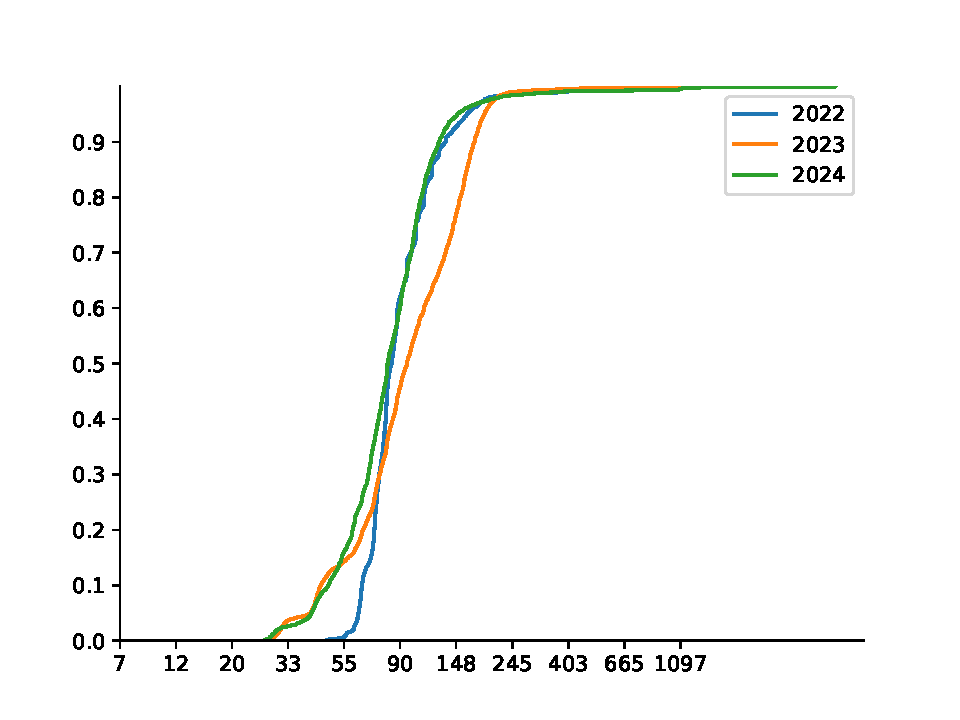
\includegraphics[width=\linewidth]{chapters/4-results/latency/img/cdf_latencies_of_starlink_probes_in_germany.pdf}
		\caption{Germany}
	\end{subfigure}
	\begin{subfigure}[b]{0.8\linewidth}
		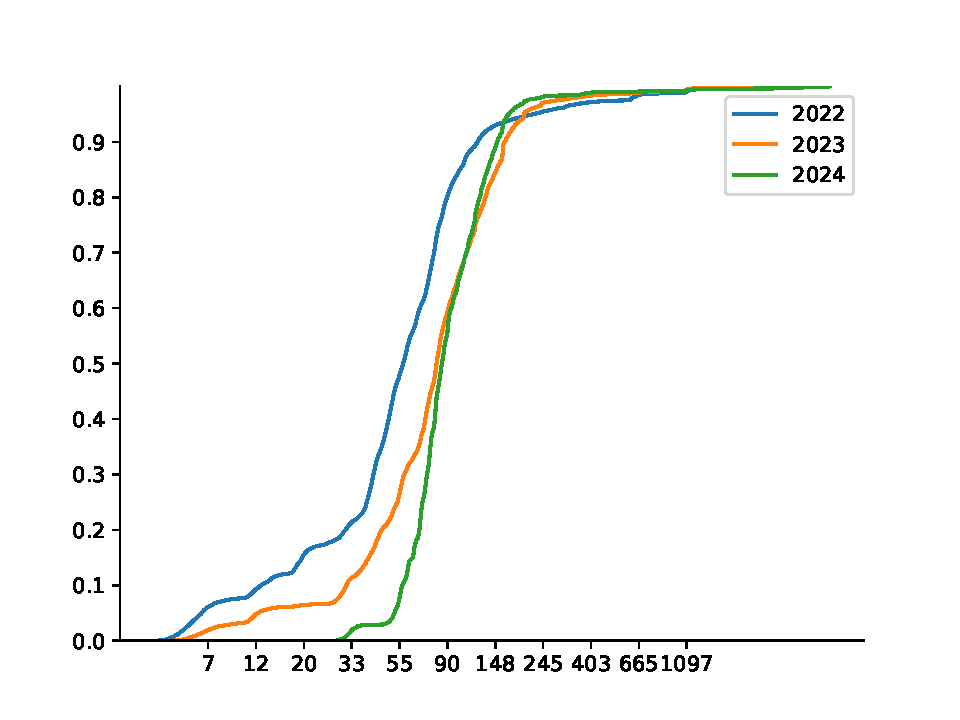
\includegraphics[width=\linewidth]{chapters/4-results/latency/img/cdf_latencies_of_starlink_probes_in_france.pdf}
		\caption{France}
	\end{subfigure}
	\caption{CDF of Latencies in Germany and France}
	\label{fig:latency-cdfs-2}
\end{figure}

\begin{figure}
	\centering
	\begin{subfigure}[b]{0.8\linewidth}
		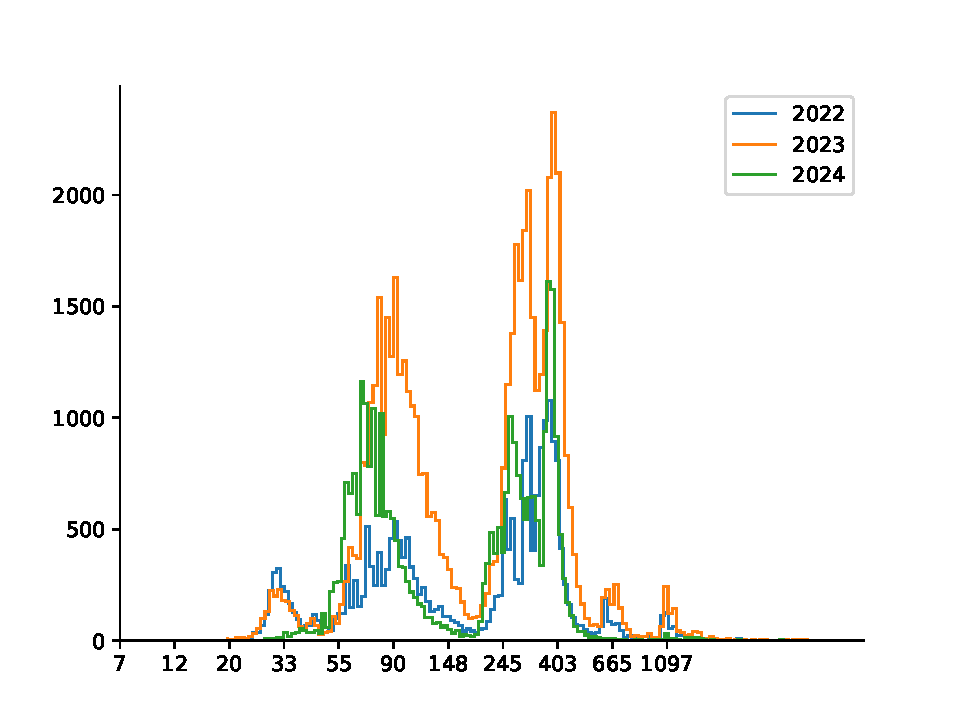
\includegraphics[width=\linewidth]{chapters/4-results/latency/img/histogram_of_latencies_of_starlink_probes_in_united_states.pdf}
		\caption{USA}
	\end{subfigure}
	\begin{subfigure}[b]{0.8\linewidth}
		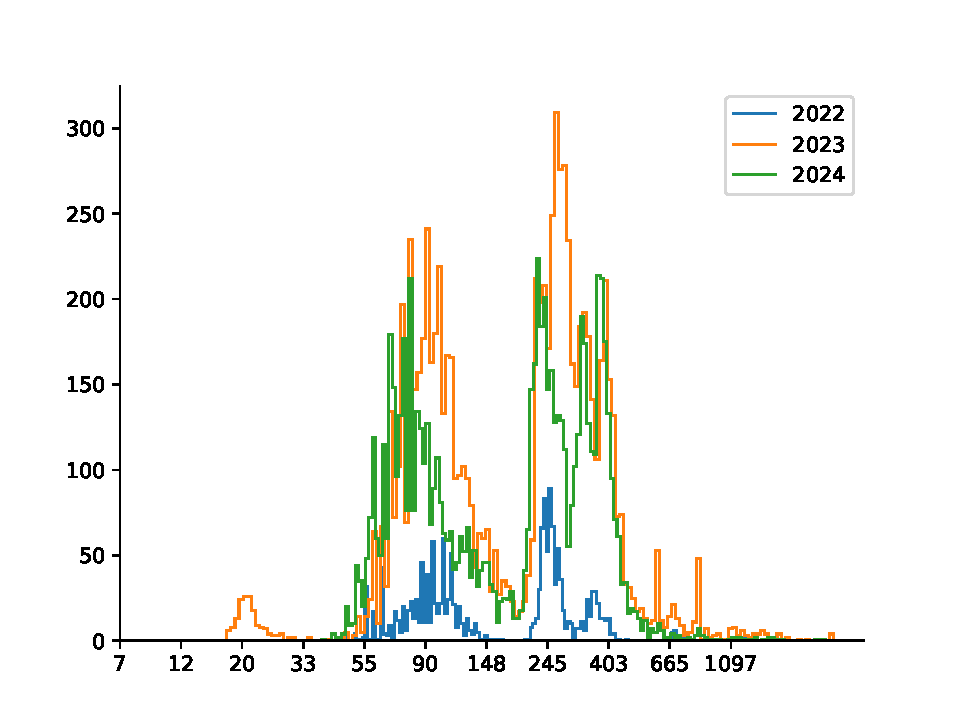
\includegraphics[width=\linewidth]{chapters/4-results/latency/img/histogram_of_latencies_of_starlink_probes_in_canada.pdf}
		\caption{Canada}
	\end{subfigure}
	\caption{EquiWidth Histogram of Latencies in the USA and Canada}
	\label{fig:latency-histogram-1}
\end{figure}

\begin{figure}
	\centering
	\begin{subfigure}[b]{0.8\linewidth}
		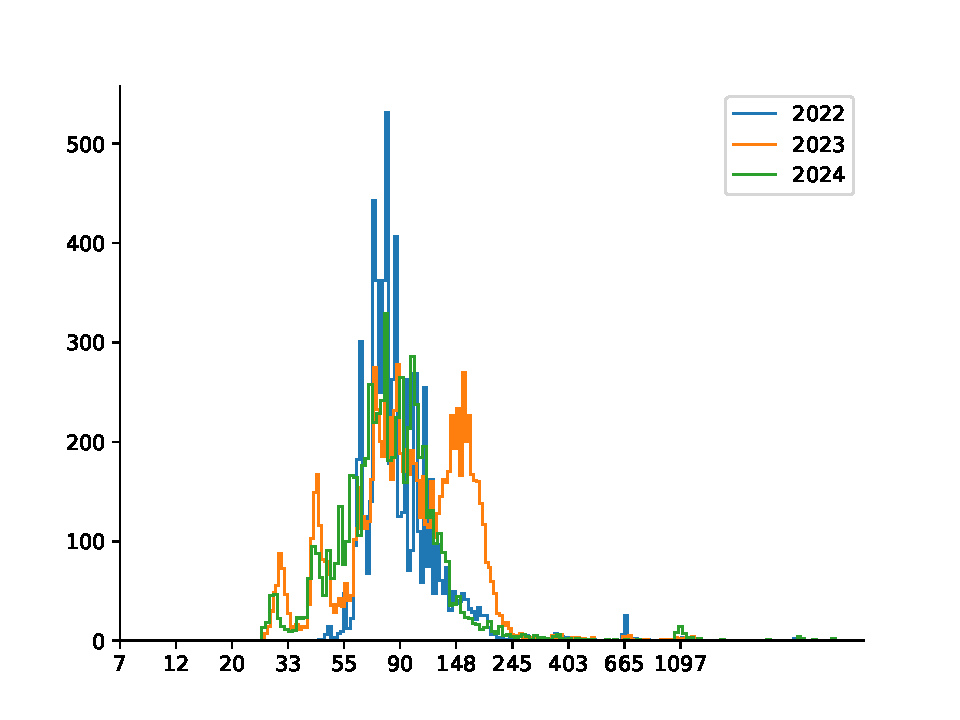
\includegraphics[width=\linewidth]{chapters/4-results/latency/img/histogram_of_latencies_of_starlink_probes_in_germany.pdf}
		\caption{Germany}
	\end{subfigure}
	\begin{subfigure}[b]{0.8\linewidth}
		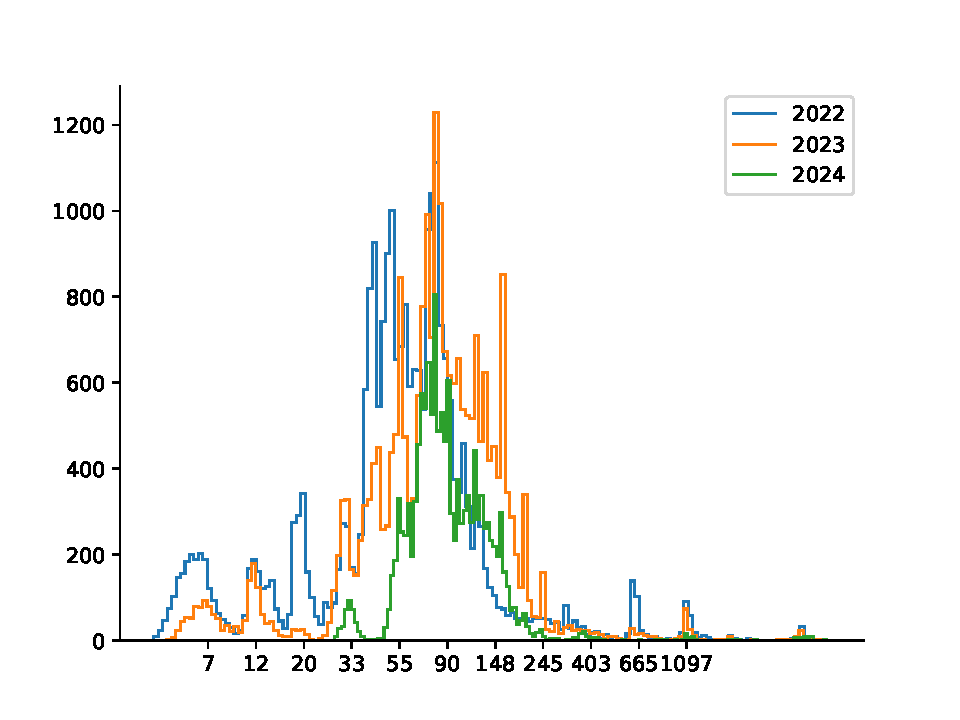
\includegraphics[width=\linewidth]{chapters/4-results/latency/img/histogram_of_latencies_of_starlink_probes_in_france.pdf}
		\caption{France}
	\end{subfigure}
	\caption{EquiWidth Histogram of Latencies in Germany and France}
	\label{fig:latency-histogram-2}
\end{figure}

Based on the assumption that Starlink does not serve all latencies equally, we
used an EquiWidth histogram\footnote{A histogram that puts all values in a
	pre-defined number of bins, where all bins cover an equally wide
	data-range.} to plot the most frequent latencies.
\Cref{fig:latency-histogram-1} and \Cref{fig:latency-histogram-2} show the
histograms for the USA, Canada, France, and Germany. It becomes apparent that
there is actually a major gap within the latencies. This gap appears for most
countries. In 2024, it became even more apparent (e.g., looking at Germany, the
gap was not visible in 2022, but appeared in 2024). For further countries, the
appendix holds further plots (see \Cref{fig:latency-cdf-3} --
\Cref{fig:latency-cdf-7} and \Cref{fig:latency-histogram-3} --
\Cref{fig:latency-histogram-7}).

Currently, it is unclear why the gap appears, but we assume that either
the measurements were consistent enough for such a pattern to occur or the gap
is a special trait of the Starlink system. The latter would infer that Starlink
serves specific latencies better than others, which means some users receive
with lower latencies in general, while others have to deal with higher
latencies. Possible causes are the weather, altitude, or \ac{GS} positioning.

Additionally, we conclude that approximately half of the measurement results
are below 100 ms, while the other half moves above 100 ms. This opposes
research suggesting Starlink performance is mostly less than 100~ms
\cite{DBLP:conf/www/MohanFCBRMO24, DBLP:conf/icnp/LaiLL20,
	DBLP:journals/pacmnet/RamanVCSZ23, DBLP:conf/imc/MichelTGB22}. Likely,
this is due to the idealized conditions research took their
measurements in, while RIPE~Atlas offers a consumer perspective.

